% \incluegraphics[width=0.95\columnwidth,height=4cm]{figures/mp-not-dead-yet.jpg}
    
\section{Introduction}\label{sec:intro}

\begin{comment}
\begin{figure}[b]
    \centering
    \captionsetup{justification=centering}
    \begin{subfigure}{0.5\columnwidth}
        \centering
        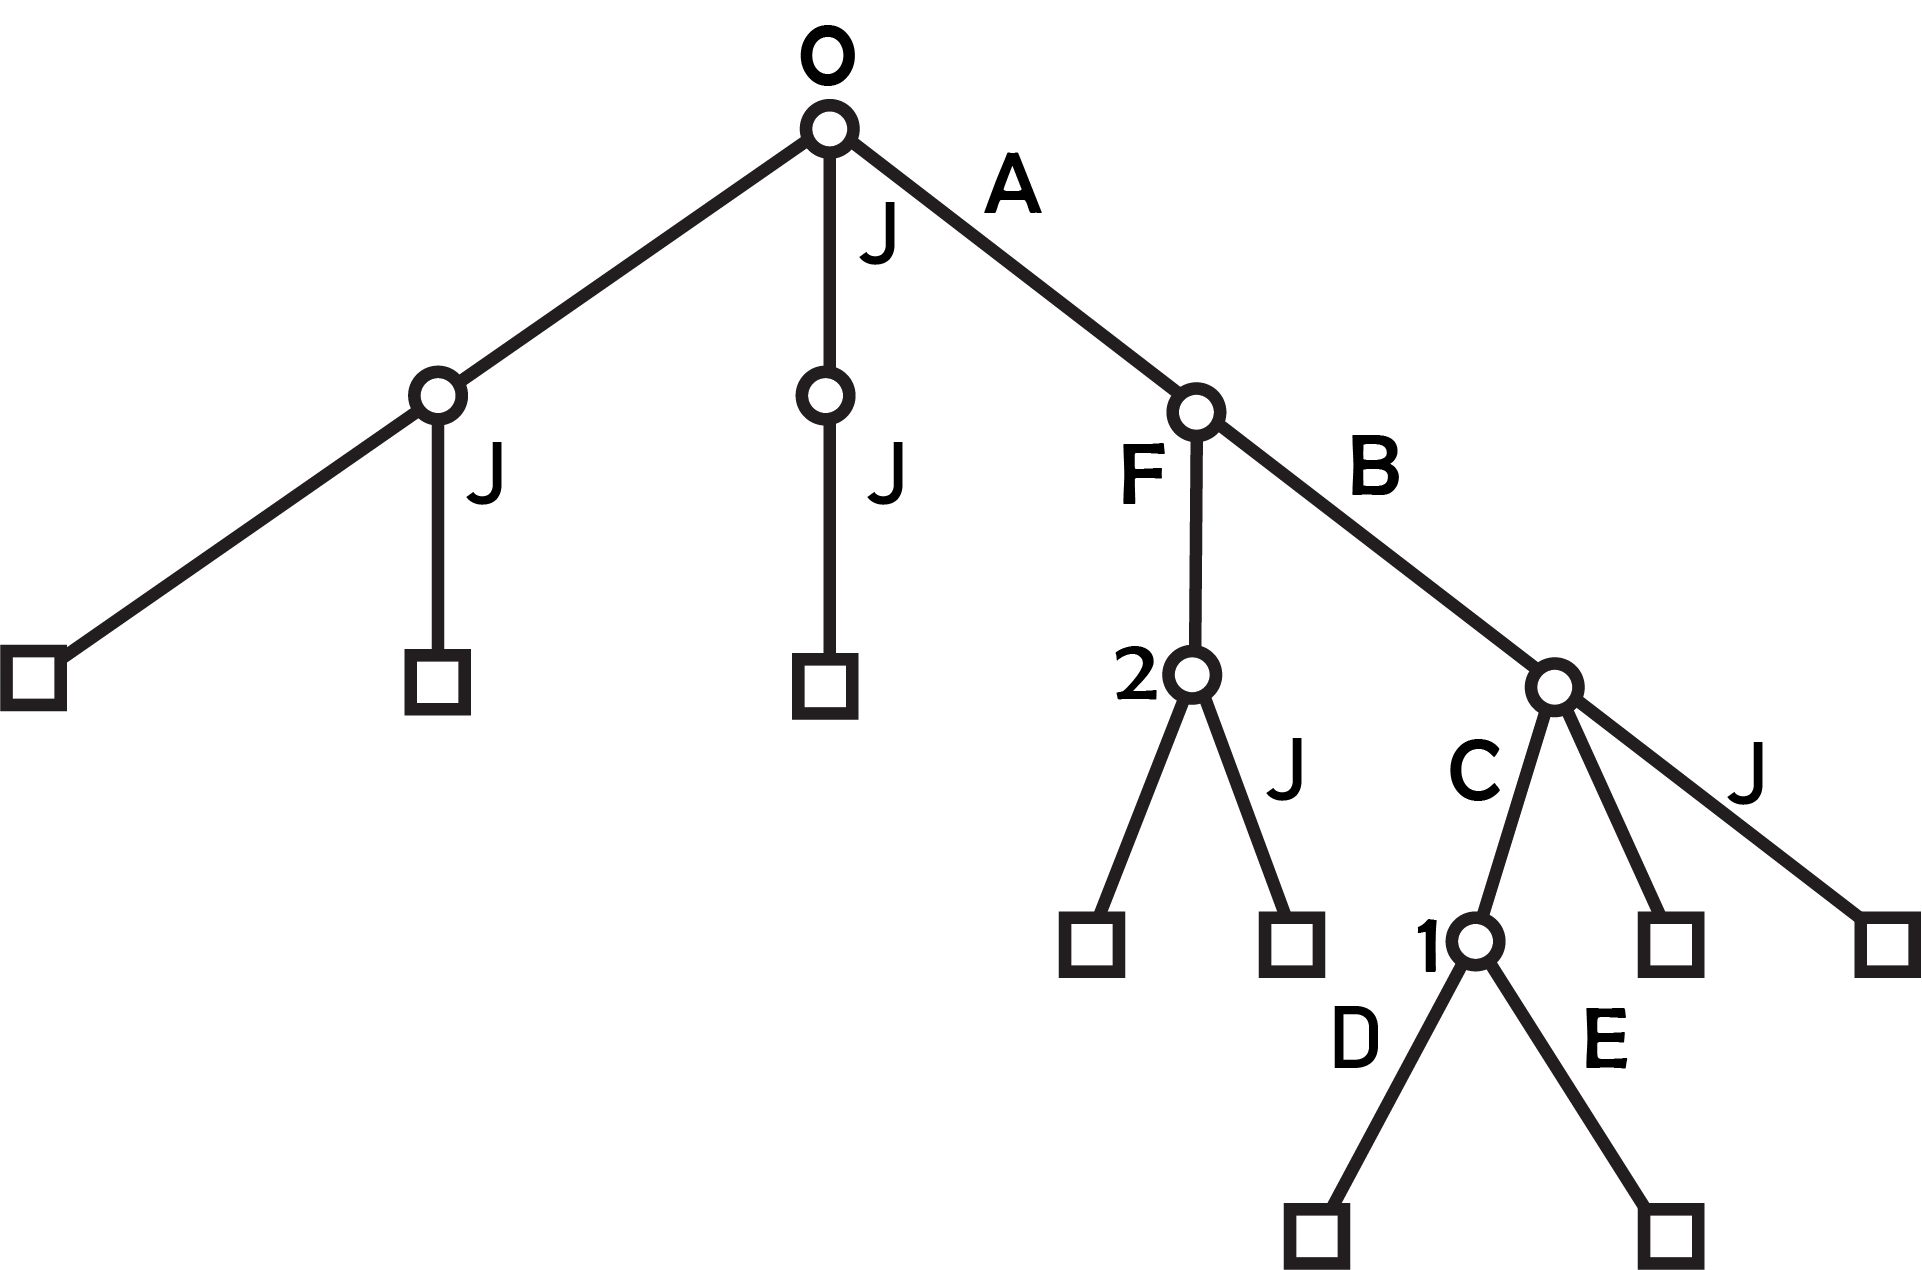
\includegraphics[width=0.95\columnwidth]{figures/multics-file-system-hierarchy-redrawn.png} 
        \caption{File System}\label{fig:hfs}
    \end{subfigure}%
    ~
    \begin{subfigure}{0.5\columnwidth}
        \centering
        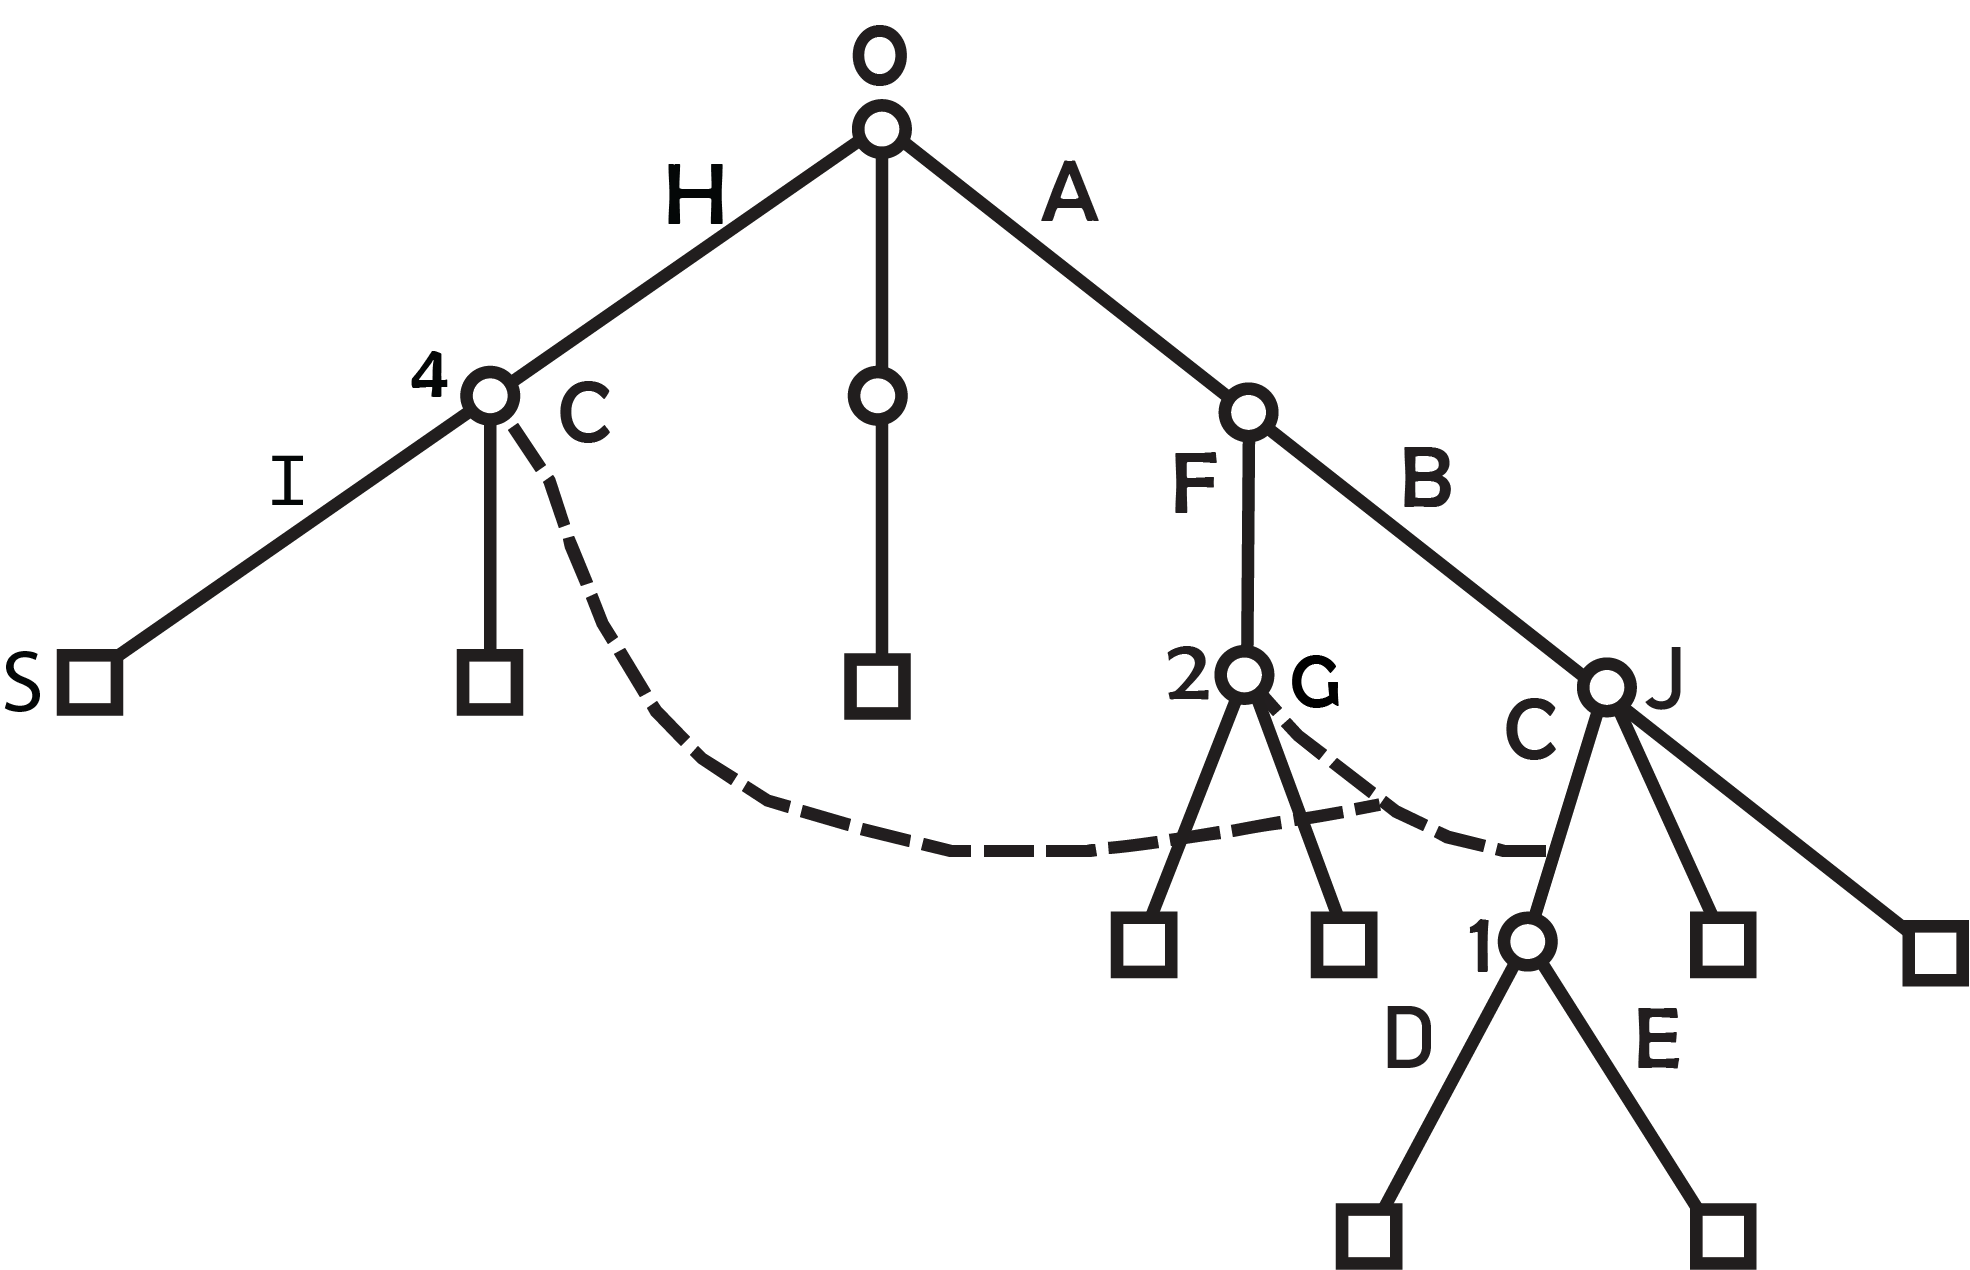
\includegraphics[width=0.95\columnwidth]{figures/multics-file-system-hierarchy-with-links-redrawn.png}
        \caption{Links Added}\label{fig:hfs-with-links}
    \end{subfigure}
    \caption{Redrawn Hierarchical File System Figures.~\cite{daley1965general}}
%    \Description{Original Multics File System Figures (redrawn) showing links.}
\end{figure}
\end{comment}

\begin{comment}
When we started using computers to store information, we chose the real-world metaphor
of physical filing systems as the basis for our design.  Thus, we had filing cabinets, 
drawers, folders, and documents.  Today, this metaphor still holds:
disk systems are cabinets;
partitions or volumes are drawers;
directories are folders; and files are documents.
However, we know there is a danger
with metaphors in computer systems~\cite{halasz1982analogy}.
\end{comment}

The hierarchical model is deeply embedded in our fundamental precepts
of data organization. Introduced in Multics~\cite{corbato1965introduction,daley1965general},
the authors describe the hierarchical file system, but they also introduce \textit{links},
suggesting an imperfect model.

Almost all systems that followed Multics adopted the hierarchical namespace, 
e.g., AT\&T~\cite{ritchie1973unix} and Digital~\cite{Spier:1973:EIK:800009.808043}.
Early UNIX work suggests limitations in the model;
they describe the importance of the \textit{permuted index server},
a program that constructed concordance databases of
file contents based upon keyword identification~\cite{ritchie1973unix}.

% Plan 9 gives us per-process name spaces~\cite{pike1992use} - but note those were part of
% other systems as well, including TENEX.

File systems, as implemented today consist of two separate components: 
the \textit{data storage} and the \textit{name space}~\cite{Seltzer2009,215e74710c2245a59b2ce117f9e74cd7,appuswamy2014building,niazi2017hopsfs}.
Data storage has evolved; gone are the days when everything a programmer
needed could be stored on a single magnetic tape or named by the numbers 1 to 2048~\cite{macdonald1956datafile,wilkes1964programmer}.
In 1965, 1TB of data required 8.4 tons of hardware; in 2019, less than 50 grams of 
media and hardware are needed.  In 2025, IDC estimates that there will be
163 zettabytes (ZB) of data~\cite{reinsel2018data}.
The namespace, however, remains fundamentally unchanged from its conceptual beginnings in
Multics; the namespace need not be tightly coupled to the underlying storage, although
it frequently is~\cite{mckusick1984fast,cao2007ext4,custer1994inside}.

The world wide web has shifted user expectations to a search-based 
model~\cite{rosenfeld2002information}.
Google revolutionized search on the internet by
leveraging metrics that exploit the inherent \emph{graph-structured} nature of the web.
Typical users think of neither  local data nor web data as hierarchical.
Some systems researchers may still employ the hierarchical mental model, but then
use ``sophisticated'' tools, such as \texttt{find} 
and \texttt{grep},, to locate relevant information in their own files --- further
evidence the file systems namespace is insufficient.
\begin{comment}
One author spent more than 20 minutes in one of our discussions of this
work searching for data they had collected in a previous study of these issues.
They had to search the local drive, multiple Google Drives, Dropbox, and
various repositories before the search was abandoned (they did eventually find
the data, but not without much pain).
\end{comment}

This is a \textit{systems} problem --- not \emph{merely} a Human Computer Interaction (HCI) 
problem ---
because the namespace belongs to the system. The system already maintains a limited
set of relationships for files, we claim that relationships
are the foundation of a better namespace model.
When starting with relationships as first class objects, the system level design
of the name space changes dramatically.

Thus, we propose a file system that natively supports relationships
as a fundamental feature. Note: the question is not \textit{should} we
be managing relationships --- we already do --- but what additional relationships
we should manage. The pure hierarchical structure is a \textit{tree}, which captures one primary relationship;
when we support an arbitrary number of equally important relationships, we
move from a \textit{tree} to a \textit{graph}.  This creates questions we consider: 1) 
How do we best capture, store, query,
and manage such relationships, and 2) How do we best present these
relationships to users.
The first is a systems problem and the subject of the rest of this paper.
The second is an HCI problem --- and one the HCI community shows considerable
interest in answering~
\cite{tunkelang2009faceted,hearst2006design,klungre2018evaluating,walton2015searching,walton2017looking,cleverley2015retrieving,huurdeman2016active,harper2013file,karlson2011version,jensen2010life,ma2009file,karger2006data,jones2005don,marsden2003improving,vicente1988accommodating,vitale2018hoarding}.

\begin{comment}
Name spaces need to...
Important ideas to capture:
Different Hierarchy over time (data science argument)
Stonebreaker: “different cuts of data”
Use case: per student notes
by project
by time
need to create CCV
Could we take a file system
Pull data out
Extract what attributes that we can automatically
Attributes:
File type
Timestamps (temporal order)
Path elements as tags
permuted indices
links
size (“find big things”)
acls
find the item (Guo) in the web cache @ same time as I wrote this e-mail?
Doc-to-e-mail.
Bibtex for files (chrome extension that downloads bibtech and paper at the same time?)
Observation: over the past 53 years we’ve made tremendous strides in terms of dealing with the storage part of file systems (e.g., journaling, log structuring, LSM, shadow versioning, distributed consensus, etc.) but we haven’t evolved the name space much at all.  The small things we have tried (extended attributes, property lists, alternate data streams/forks) haven’t gained much traction. Why is this the case?
\end{comment}

\begin{comment}
REFERENCES
https://venturebeat.com/wp-content/uploads/2013/01/6a00e009844716883300e55412e9c98834-800wi.jpg
corbato1965introduction (Multics)
ritchie1973unix
https://www.seagate.com/www-content/our-story/trends/files/Seagate-WP-DataAge2025-March-2017.pdf
Russell and Norvig, AIMA
\end{comment}

